%-------------------------------------------------------------
\subsection{Example 5} \label{sec:ch5:example5}

%-------------------------------------------------------------
\subsubsection{Description}

The final example is a constructed problem that will help demonstrate some of the problem elements and extensions in Sec.~\ref{sec:ch5:extensions} not seen in the previous examples.
The infinite-dimensional problem formulation is:%
\allowdisplaybreaks[1]%
\begin{subequations}%%
\begin{align}
\min_{\bm{u}(t)} \quad & \int_0^1 \left[ u_1^2/10 + u_2^2/10 + u_1\xi_1 + u_1\xi_2 + 5\left(\xi_2-g(t)\right)^2 \right] dt + \max_{0\leq t\leq 1} \xi_3(t) \\
\text{subject to:} \quad & \dot{\bm{\xi}} = \begin{bmatrix} -1 & 2 & 0 \\ 3 & -4 & 0 \\ 1 & 2 & -1 \end{bmatrix} \bm{\xi} +
\begin{bmatrix} 1 & 0 \\ -1 & 0 \\ 0 & 1/20 \end{bmatrix} \bm{u} \\
& \xi_1(0) = 2, \quad \xi_3(0) = 1/2 \\
& \xi_2(0) - \xi_2(1) = 0 \\
& \int_0^1 \xi_1(t) dt = 0 \\
& -\xi_1(t) + u_2(t)/12 \leq 0 \\
& \xi_2(t) \leq g(t) \\
& \abs{u_2} \leq 10 
\end{align}
\end{subequations}%%
\allowdisplaybreaks[0]%

\noindent where 
$5\left(\xi_2-g(t)\right)^2$ is an output tracking term (resulting in time-varying quadratic, linear, and constant objective function terms, see Sec.~\ref{sec:ch5:output}),
$\max\xi_3(t)$ is a min-max objective term (that will be approximated with a parameter, see Sec.~\ref{sec:ch5:minmax:objective}),
$\xi_2(0) - \xi_2(1) = 0$ is a periodic constraint (that will be implemented as a linear equality constraint),
$\int_0^1 \xi_1(t) dt = 0$ is an integral constraint (which will be approximated with an additional state, see Sec.~\ref{sec:ch5:integral:constraints}),
$-\xi_1(t) + u_2(t)/12 \leq 0$ is a mixed control-state path constraint,
$\xi_2(t) \leq g(t) $ is a time-varying simple bound,
and
$\abs{u_2} \leq 10 $ is a linear absolute value constraint (that will be implemented with two constraints, see Sec.~\ref{sec:ch5:absolute:values}).
For brevity, the structure-based implementation is only shown in the \textsc{Matlab} code in Sec.~\ref{sec:ex5-code}. 

%-------------------------------------------------------------
\subsubsection{Solution}

This example, like many \lqdo{} problems, does not have a straightforward solution, so we can instead use \dt{} to obtain an approximate solution.
Here we set $g(t) = \sin(2 \pi t) +1/2$.
The optimal trajectories for the states and controls are shown in Fig.~\ref{fig:ch5:ex5sens} along with the trajectories for the integral and mixed control-state constraints.
This solution was found using ED-HS-CQHS (5) with 5,000 node points and $\Psi^*=6.368153$.
All constraints are satisfied, and all the path constraints enter and exit activity during the time horizon.

\begin{figure}
\centering

\begin{subfigure}{0.5\textwidth}
\centering
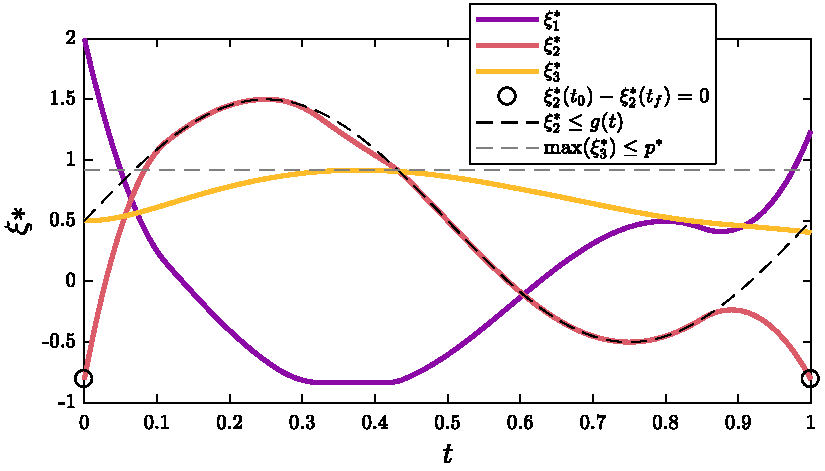
\includegraphics[width=\textwidth]{../ch5/figures/ex5sol-states}%
\caption{States.}
\label{fig:ch5:ex5sol:states}
\end{subfigure}%
\begin{subfigure}{0.5\textwidth}
\centering
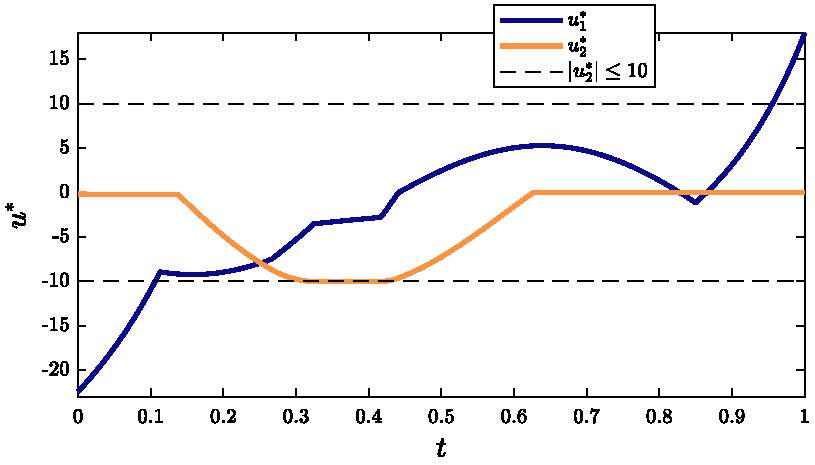
\includegraphics[width=\textwidth]{../ch5/figures/ex5sol-controls}%
\caption{Controls.}
\label{fig:ch5:ex5sol:controls}
\end{subfigure}%

\begin{subfigure}{\textwidth}
\centering
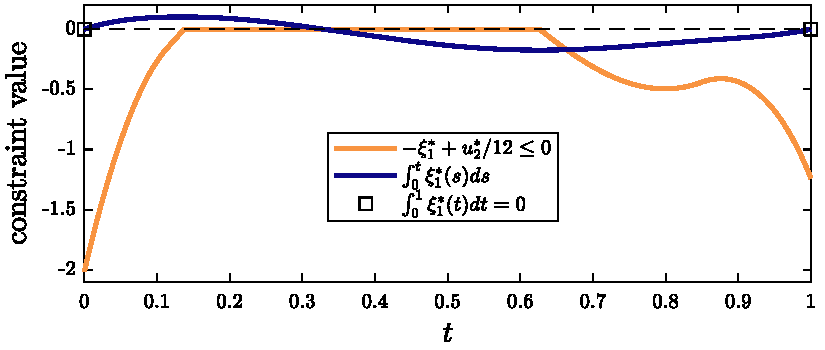
\includegraphics[width=0.5\textwidth]{../ch5/figures/ex5sol-other}%
\caption{Integral and mixed state-control path constraints.}
\label{fig:ch5:ex5sol:other}
\end{subfigure}%

\caption{Solution for \nameref{sec:ch5:example5}.}
\label{fig:ch5:ex5sens}
\end{figure}